\chapter{Funciones complejas y mapeo}

\unsection{Introducción}
Una función compleja tiene dominio e imagen en 2 dimensiones ya que toma un numero complejo y lo transforma en otro numero complejo. Lo que quiere decir esto es que las funciones complejas tienen 2 variables independientes y 2 variables dependientes. Por esta cualidad para graficarlas correctamente necesitaríamos un sistema de representación en 4 dimensiones, 2 para las variables y otras 2 para las respuestas, lo cual es físicamente imposible. Otra forma de poder visualizar como se comportan las funciones complejas es graficar como se modifica el plano complejo a través de una función y otra forma es tomar elementos geométricos, como lineas y círculos y ver como son transformadas por la función. Llegar a poder visualizar como se comportan distintas funciones a través de este concepto es el objetivo de esta parte de la materia.

\unsection{Ecuación complejas}
Antes de saltar a funciones y mapeos deberíamos definir como funcionan las ecuaciones complejas. Una ecuación compleja se define de manera similar a una ecuación de una variable. La variable compleja se le sule denotar con una $z$. Una ecuación de ejemplo seria:
\begin{equation}\label{eq:ejmEQC}
    z^2+3=0
\end{equation}
Como en una ecuación de numero reales, el conjunto solución de la ecuación \ref{eq:ejmEQC} son todos aquellos números complejo que satisfagan la igualdad. En este caso es una ecuación de orden 2 así que vamos a obtener 2 respuestas. Los método de resolución aplicables son iguales al de una ecuación real, usando la formula de baskara por ejemplo o despejando $z$ para encontrar la condición que debe cumplir la variable. Partiendo de la ecuación \ref{eq:ejmEQC}:
\begin{equation}\label{eq:ejmEQCS1}
    \begin{aligned}
         z^2+3=0 \lrah z^2&=-3\\
                        \pm z&=\sqrt{-3}\\
                        z&=\pm \sqrt{-1\cdot 3}\\
                        z&=\pm \sqrt{-1}\cdot\sqrt{3}\\
                        z&=\pm j\sqrt{3}
    \end{aligned}
\end{equation}
A diferencia de las ecuaciones reales la incógnita $z$ es una incógnita de 2 dimensiones($z=x+jy$), por lo tanto una ecuación compleja puede subdividirse en la parte que restringe los valores reales y otra que rige los valores posibles de la parte imaginaria de $z$. Haciendo el planteo desde la ecuación \ref{eq:ejmEQC}:
\begin{equation}
    \begin{aligned}
     z^2+3=0 \lrah &(x+jy)^2+3=0\\
                      &(x+jy)\cdot(x+jy)=-3\\
                  &(x^2+(jy)^2)+(x\cdot jy + x\cdot jy)=-3
    \end{aligned}
\end{equation}
\begin{equation}
    (x^2-y^2)+j(2xy)=(-3\ ,\ j0)
\end{equation}
De aquí podemos separa la parte real de la respuesta con la parte real de la incógnita y lo mismo con las partes imaginarias, generando un sistema de ecuación.
\begin{equation}
(x^2-y^2)+j(2xy)=(-3\ ,\ j0)
    \begin{cases}
        x^2-y^2=-3\\
        2xy=0
    \end{cases}
\end{equation}
Resolviendo el sistema de ecuaciones llegaremos a la conclusión de que $x=0$ y $y=\pm \sqrt{3}$, recordando que $z=x+jy$ llegaremos a la misma solución que en la ecuación \ref{eq:ejmEQCS1}:
\begin{equation}
\begin{aligned}
    (x=0\ ;\ y=\pm \sqrt{3})\lrah z&=(x+jy)\\
                                z&=(0+j(\pm\sqrt{3})\\
                                z&=\pm j\sqrt{3}
\end{aligned}
\end{equation}

\unsection{Parametrización de curvas}
Para poder mapear funciones complejas debemos ser capaces de generar elementos geométricos en el plano complejo a través de una ecuación que describa su comportamiento. 

El método general para crear una ecuación que describa una curva es plantear un numero complejo genérico en alguna de sus formas y dejar como constante alguna de sus partes, ya se la parte real, imaginaria, modulo o argumento y hacer variable la otra parte. Modificando el intervalo en el que la parte variable existe  seremos capaces de construir arcos, semi-rectas, etc.
\unsubsection{Lineas verticales y horizontales}
\unsubsubsection{Linea horizontal}
En el plano de 2 dimensiones reales una linea horizontal es el lugar geométrico en el cual los puntos pertenecientes al mismo posen la misma coordenada constante en $y$, generando una recta perpendicular al eje $x$.
\begin{equation}
    (x,y)\begin{cases}
        y=c\\
        x=t
    \end{cases}
\end{equation}
De manera similar una recta horizontal en el plano complejo esta descripta por la siguiente ecuación:
\begin{equation}\label{eq:DeflhF}
    z=t+j\kappa
\end{equation}
$\kappa$ siendo una constate y $t$ siendo variable.
\begin{figure}[H]
    \centering
    \begin{minipage}{0.45\textwidth}
        \centering
        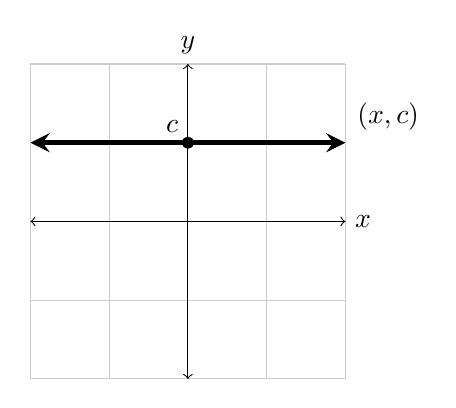
\begin{tikzpicture}
    \draw[thin,gray!40] (-2,-2) grid (2,2);
    \draw[<->] (-2,0)--(2,0) node[right] {$x$};
    \draw[<->] (0,-2)--(0,2) node[above]{$y$};
    \draw[fill=black] (0,1) circle(2pt) node[anchor=south east]{$c$};
    \draw[line width=2pt,black,stealth-stealth] (-2,1)--(2,1) node[anchor=south west]{$(x,c)$};
\end{tikzpicture}
\caption*{Linea horizontal real}
    \end{minipage}
    \begin{minipage}{0.45\textwidth}
        \centering
        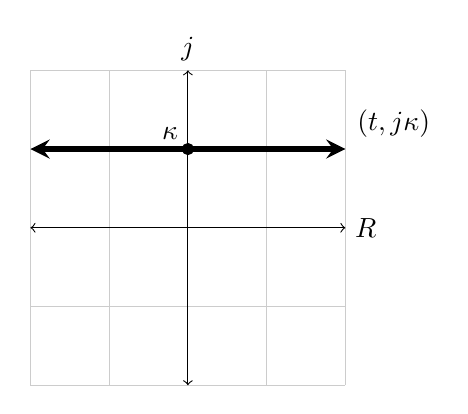
\begin{tikzpicture}
    \draw[thin,gray!40] (-2,-2) grid (2,2);
    \draw[<->] (-2,0)--(2,0) node[right] {$R$};
    \draw[<->] (0,-2)--(0,2) node[above]{$j$};
    \draw[fill=black] (0,1) circle(2pt) node[anchor=south east]{$\kappa$};
    \draw[line width=2pt,black,stealth-stealth] (-2,1)--(2,1) node[anchor=south west]{$(t,j\kappa)$};
\end{tikzpicture}
\caption*{Linea horizontal compleja}
    \end{minipage}
    \caption{}
    \label{fig:ComLHF}
\end{figure}
Restringido los valores que pude tomar $x$ podremos genera segmentos horizontales.

\unsubsubsection{Linea vertical}
En el plano de 2 dimensiones reales una linea vertical es el lugar geométrico en el cual los puntos pertenecientes al mismo posen la misma coordenada constante en $x$, generando una recta perpendicular al eje $y$.
\begin{equation}
    (x,y)\begin{cases}
        y=t\\
        x=c
    \end{cases}
\end{equation}
De manera similar una recta horizontal en el plano complejo esta descripta por la siguiente ecuación:
\begin{equation}\label{eq:DeflvF}
    z=\kappa+jt
\end{equation}
$\kappa$ siendo una constate y $t$ siendo variable.
\begin{figure}[H]
    \centering
    \begin{minipage}{0.45\textwidth}
        \centering
        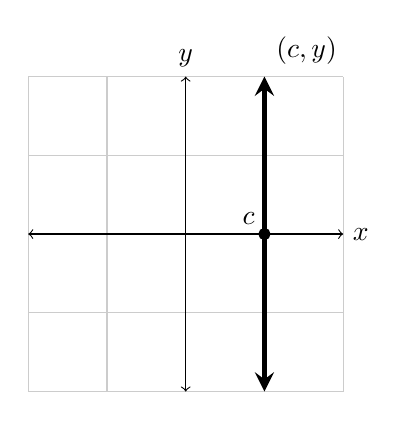
\begin{tikzpicture}
    \draw[thin,gray!40] (-2,-2) grid (2,2);
    \draw[<->] (-2,0)--(2,0) node[right] {$x$};
    \draw[<->] (0,-2)--(0,2) node[above]{$y$};
    \draw[fill=black] (1,0) circle(2pt) node[anchor=south east]{$c$};
    \draw[line width=2pt,black,stealth-stealth] (1,-2)--(1,2) node[anchor=south west]{$(c,y)$};
\end{tikzpicture}
\caption*{Linea vertical real}
    \end{minipage}
    \begin{minipage}{0.45\textwidth}
        \centering
        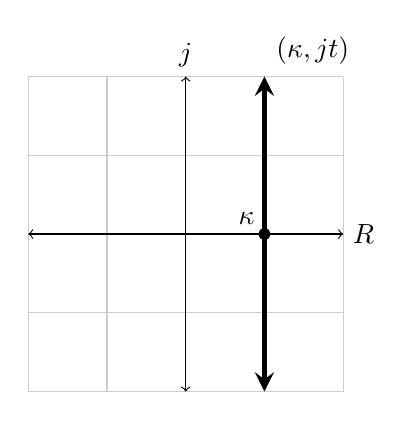
\begin{tikzpicture}
    \draw[thin,gray!40] (-2,-2) grid (2,2);
    \draw[<->] (-2,0)--(2,0) node[right] {$R$};
    \draw[<->] (0,-2)--(0,2) node[above]{$j$};
    \draw[fill=black] (1,0) circle(2pt) node[anchor=south east]{$\kappa$};
    \draw[line width=2pt,black,stealth-stealth] (1,-2)--(1,2) node[anchor=south west]{$(\kappa,jt)$};
\end{tikzpicture}
\caption*{Linea vertical compleja}
    \end{minipage}
    \caption{}
    \label{fig:ComVHF}
\end{figure}
Restringido los valores que pude tomar $y$ podremos genera segmentos verticales.
\unsubsubsection{Rectángulos}
Ahora que definimos como parametrizar lineas horizontales y verticales, podemos crear cuadrados y rectángulos en el plano complejo. Por ejemplo planteamos un rectángulo que tenga por vértices los puntos $\ a=(1+j)$; $\ b=(3+j)$; $\ c=(3+j2)$; $d\ =(1+2j)$, entonces el rectángulo estará conformado por los segmentos horizontales, $\overline{ab}$ y $\overline{cd}$, y los segmentos verticales $\overline{bc}$ y $\overline{da}$. Los segmentos horizontales estarán dados entonces por:
\begin{equation}
\begin{aligned}
    \overline{ab}=(x+jy)&
    \begin{cases}
        x=\Real{a}\leq t\leq\Real{b}\lrah x=1\leq t\leq 3\\
        y=\Imag{a}=\Imag{b}\lrah y=1
    \end{cases}\\
    \\
    \overline{cd}=(x+jy)&
    \begin{cases}
        x= \Real{c}\leq t\leq\Real{d}\lrah x=1\leq t\leq 3\\
        y=\Imag{a}=\Imag{b} \lrah y=2
    \end{cases}
\end{aligned}
\end{equation}
y los segmentos verticales estarán dados por:
\begin{equation}
\begin{aligned}
    \overline{bc}=(x+jy)&
    \begin{cases}
        x=\Real{c}=\Real{d}\lrah x=3\\
        y=\Imag{b}\leq t\leq \Imag{c}\lrah y=1\leq t\leq2
    \end{cases}\\
    \\
    \overline{da}=(x+jy)&
    \begin{cases}
        x=\Real{d}=\Real{a}\lrah x=1\\
        y=\Imag{b}\leq t\leq \Imag{c}\lrah y=1\leq t\leq2
    \end{cases}
\end{aligned}
\end{equation}
Obteniendo la expresión del rectángulo.
\begin{figure}[H]
    \centering
    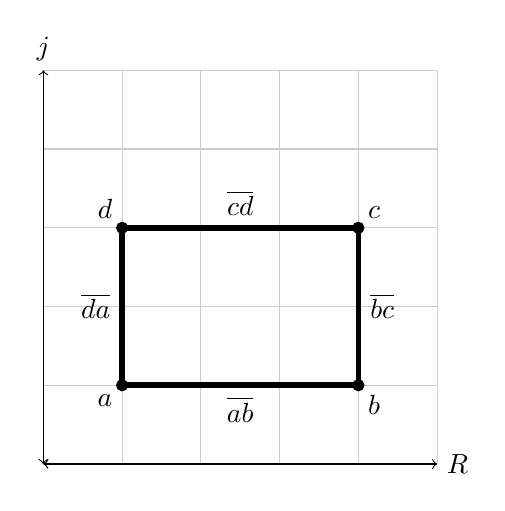
\begin{tikzpicture}
    \draw[thin,gray!40] (0,0) grid (5,5);
    \draw[<->] (0,0)--(5,0) node[right] {$R$};
    \draw[<->] (0,0)--(0,5) node[above]{$j$};
    \coordinate (a) at (1,1);
    \coordinate (b) at (4,1);
    \coordinate (c) at (4,3);
    \coordinate (d) at (1,3);
    
    \draw[fill=black] (a) circle(2pt) node[anchor=north east]{$a$};
    \draw[fill=black] (b) circle(2pt) node[anchor=north west]{$b$};
    \draw[fill=black] (c) circle(2pt) node[anchor=south west]{$c$};
    \draw[fill=black] (d) circle(2pt) node[anchor=south east]{$d$};
    
    \draw[line width=2pt,black,-] (a)--(b) node[midway, below]{$\overline{ab}$};
    \draw[line width=2pt,black,-] (b)--(c) node[midway, right]{$\overline{bc}$};
    \draw[line width=2pt,black,-] (c)--(d) node[midway, above]{$\overline{cd}$};
    \draw[line width=2pt,black,-] (d)--(a) node[midway, left]{$\overline{da}$};
    
\end{tikzpicture}
\caption{Rectángulo en el plano complejo con lineas parametrizadas}
    \label{fig:RectF}
\end{figure}
\unsubsection{Superficies}
Para definir una superficie tomamos como una linea horizontal o vertical, entonces la expresión:
\begin{equation}
    \Real{z} \geq \kappa
\end{equation}
define la superficie $S$ descripta en la figura \ref{fig:SupVF}:
\begin{figure}[H]
    \centering
    \begin{tikzpicture}
    \draw[thin,gray!40] (-2,-2) grid (2,2);
    \draw[<->] (-2,0)--(2,0) node[right] {$R$};
    \draw[<->] (0,-2)--(0,2) node[above]{$j$};
    \filldraw[draw=gray!40, fill=mlgb, fill opacity=0.6] (0.5,-2) -- (0.5,2) -- (2,2) -- (2,-2);
    \draw[line width=2pt,black,-] (0.5,-2)--(0.5,2);
    \draw[fill=black] (0.5,0) circle(2pt) node[anchor=south east]{$\kappa$};
    \draw[] (1.20,0) node[above]{$S$};
\end{tikzpicture}
\caption{Superficie $S$}
    \label{fig:SupVF}
\end{figure}
De manera similar la ecuación:
\begin{equation}
    \Imag{z} \geq \kappa
\end{equation}
define la superficie $S$ de la figura \ref{fig:SupHF}:
\begin{figure}[H]
    \centering
    \begin{tikzpicture}
    \draw[thin,gray!40] (-2,-2) grid (2,2);
    \draw[<->] (-2,0)--(2,0) node[right] {$R$};
    \draw[<->] (0,-2)--(0,2) node[above]{$j$};
    \filldraw[draw=gray!40, fill=mlgb, fill opacity=0.6] (-2,-0.5) -- (2,-0.5) -- (2,2) -- (-2,2);
    \draw[line width=2pt,black,-] (-2,-0.5)--(2,-0.5);
    \draw[fill=black] (0,-0.5) circle(2pt) node[anchor=north east]{$\kappa$};
    \draw[] (0,1.2) node[right]{$S$};
\end{tikzpicture}
\caption{Superficie $S$}
    \label{fig:SupHF}
\end{figure}
\unsubsection{Rectas, semi-rectas y segmentos}
Una recta, en un espacio de 2 dimensiones reales, de ordenada al origen igual al punto $(0,0)$ esta formada por infinitos puntos que satisfagan la condición:
\begin{equation}
   y=x\cdot a \lrah \frac{x}{y}=a
\end{equation}
$a$ siendo una constante arbitraria y $(x\ ,\ y)$ siendo los componentes de los puntos. Si trazamos una linea con cada uno de nuestros punto hasta la ordenada de origen veremos que todas las lineas generan una ángulo de $\tan^{-1}{(\frac{y}{x})}$ con respecto al eje $x$. Ya que $x$ e $y$ son proporcionales entre ellos por un factor $a$, por como se define una recta, todos los puntos poseerán el mismo ángulo con respecto al eje $x$.

En el plano complejo una recta debe comportarse de una manera similar, todos los puntos pertenecientes a la recta deben tener el mismo ángulo o argumento, entonces recordando la definición exponencial de un numero complejo \ref{eq:defExp} podemos definir una recta como un numero complejo de argumento constante $\gamma$ y modulo variable $r$:
\begin{equation}\label{eq:DefRectF}
    z_{(r)}=re^{j\gamma}\llrah \ z_{(r)}=r\cdot[\cos{(\gamma)}+j\sen{(\gamma)}] 
\end{equation}
\begin{figure}[H]%
\centering
    \begin{minipage}{0.5\textwidth}
    \centering
        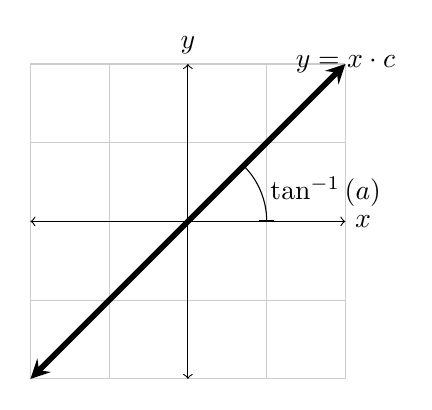
\begin{tikzpicture}
    \draw[thin,gray!40] (-2,-2) grid (2,2);
    \draw[<->] (-2,0)--(2,0) node[right] {$x$};
    \draw[<->] (0,-2)--(0,2) node[above]{$y$};
    \draw[line width=2pt,black,stealth-stealth] plot[smooth,domain=-2:2] (\x, {\x}) node[]{$y=x\cdot c$};
    \draw[|-|] (1,0) arc (0:45:1) node [midway, right]{$\tan^{-1}{(a)}$};
\end{tikzpicture}
\caption*{Recta real}
    \end{minipage}%
    \begin{minipage}{0.4\textwidth}
    \centering
        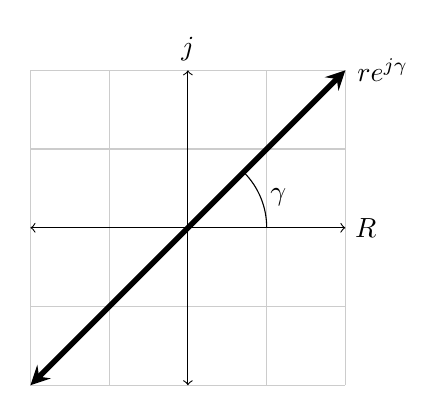
\begin{tikzpicture}
    \draw[thin,gray!40] (-2,-2) grid (2,2);
    \draw[<->] (-2,0)--(2,0) node[right] {$R$};
    \draw[<->] (0,-2)--(0,2) node[above]{$j$};
    \draw[line width=2pt,black,stealth-stealth] plot[smooth,domain=-2:2] (\x, {\x}) node[right]{$re^{j\gamma}$};
    \draw[|-|] (1,0) arc (0:45:1) node [midway, right]{$\gamma$};
\end{tikzpicture}
\caption*{Recta en el plano complejo}
    \end{minipage}%
    \caption{Comparación entre un numero complejo y un vector de 2 dimensiones reales}
    \label{fig:compRectasF}
\end{figure}
En la forma polar de la expresión \ref{eq:DefRectF} se pude ver claramente que, al ser $\gamma$ una constante, el coseno y el seno son también constantes, entonces la parte real e imaginaria siempre van a ser proporcionales a $r$ manteniendo la relación $\frac{\Real{z}}{\Imag{z}}$ constante.
Modificando el intervalo en el que varia $r$ seremos capaces de crear distintos objetos geométricos
\begin{figure}[H]
\centering
    \begin{minipage}{0.3\textwidth}
        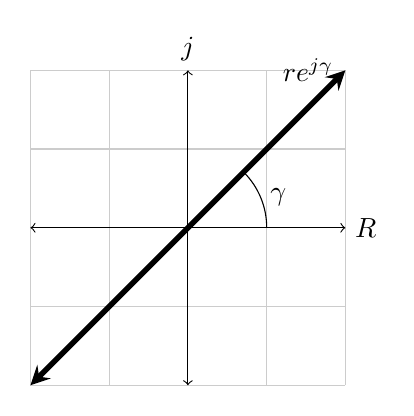
\begin{tikzpicture}
    \draw[thin,gray!40] (-2,-2) grid (2,2);
    \draw[<->] (-2,0)--(2,0) node[right] {$R$};
    \draw[<->] (0,-2)--(0,2) node[above]{$j$};
    \draw[line width=2pt,black,stealth-stealth] plot[smooth,domain=-2:2] (\x, {\x}) node[left]{$re^{j\gamma}$};
    \draw[|-|] (1,0) arc (0:45:1) node [midway, right]{$\gamma$};
\end{tikzpicture}
\caption*{Recta: $-\infty< r <\infty$}
    \end{minipage}
    \begin{minipage}{0.3\textwidth}
        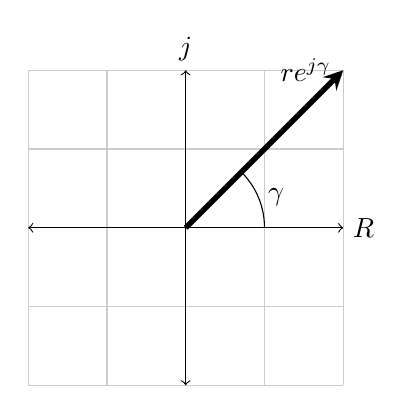
\begin{tikzpicture}
    \draw[thin,gray!40] (-2,-2) grid (2,2);
    \draw[<->] (-2,0)--(2,0) node[right] {$R$};
    \draw[<->] (0,-2)--(0,2) node[above]{$j$};
    \draw[line width=2pt,black,-stealth] plot[smooth,domain=0:2] (\x, {\x}) node[left]{$re^{j\gamma}$};
    \draw[|-|] (1,0) arc (0:45:1) node [midway, right]{$\gamma$};
\end{tikzpicture}
\caption*{Semi-recta: $0\leq r <\infty$}
    \end{minipage}
    \begin{minipage}{0.3\textwidth}
        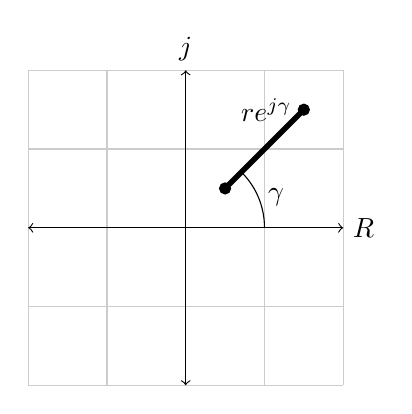
\begin{tikzpicture}
    \draw[thin,gray!40] (-2,-2) grid (2,2);
    \draw[<->] (-2,0)--(2,0) node[right] {$R$};
    \draw[<->] (0,-2)--(0,2) node[above]{$j$};
    \draw [fill=black] (0.5,0.5) circle(2pt);
    \draw [fill=black] (1.5,1.5) circle(2pt);
    \draw[line width=2pt,black,-] plot[smooth,domain=0.5:1.5] (\x, {\x}) node[left]{$re^{j\gamma}$};
    \draw[|-|] (1,0) arc (0:45:1) node [midway, right]{$\gamma$};
\end{tikzpicture}
\caption*{Segmento: $a\leq r \leq b$}
    \end{minipage}
    \caption{}
    \label{fig:RectaExpoF}
\end{figure}
También podemos desplazar la recta sumándole cualquier numero complejo fijo como constante. Entonces la ecuación general de una recta en el plano complejo seria:
\begin{equation}
    z_{(r)}=re^{j\gamma}+z_c \llrah\ z_{(r)}=r\cdot[\cos{(\gamma)}+j\sen{(\gamma)}]+z_c
\end{equation}
\begin{figure}[H]
    \centering
    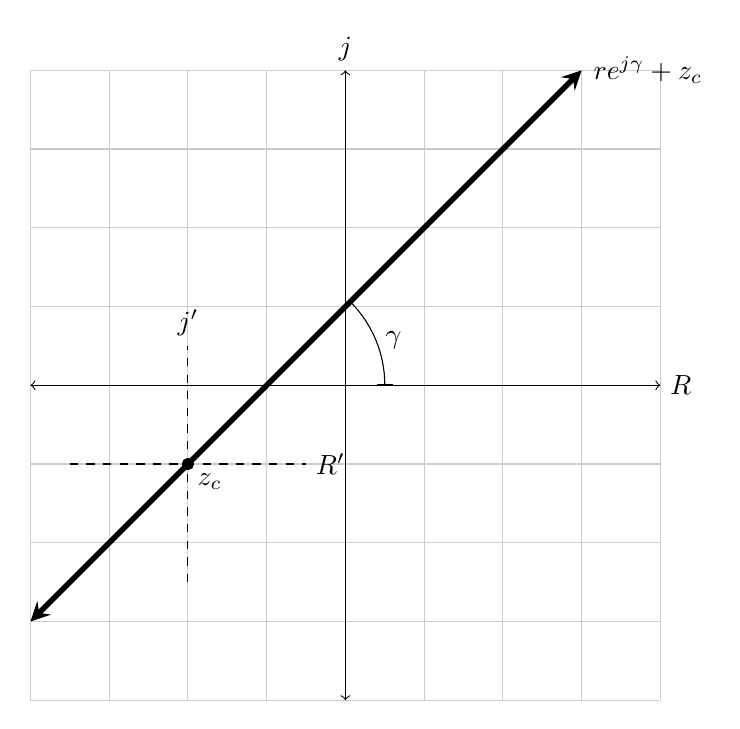
\begin{tikzpicture}
    \draw[thin,gray!40] (-4,-4) grid (4,4);
    \draw[<->] (-4,0)--(4,0) node[right] {$R$};
    \draw[<->] (0,-4)--(0,4) node[above]{$j$};
    \draw[dashed] (-3.5,-1)--(-0.5,-1) node[right] {$R'$};
    \draw[dashed] (-2,-2.5)--(-2,0.5) node[above]{$j'$};
    \draw [fill=black] (-2,-1) circle(2pt) node[anchor=north west]{$z_c$};
    \draw[line width=2pt,black,stealth-stealth] plot[smooth,domain=-4:3] (\x, {\x+1}) node[right]{$re^{j\gamma}+z_c$};
    \draw[|-|] (0.5,0) arc (0:45:1.5) node [midway, right]{$\gamma$};
\end{tikzpicture}
\caption{Recta genérica desplazada un $z_c$}
\end{figure}
Al sumar un numero complejo $z_c$ es como si estuviéramos desplazando los ejes coordenados al punto $z_c$ ya que cuando $r=0$
estaríamos parado en el centro de este nuevo sistema de ejes coordenado desplazado relativamente al antiguo eje coordenado, como si fuera una transformación lineal. La base de este nuevo sistema coordenado seria la base desplazada en $z_c$, $\ j'=j+z_c$ y $\ R'=1+z_c$. Esto ultimo no es muy relevante pero sienta las bases para ver como funciona un desplazamiento en una función compleja.

De la ecuación \ref{eq:DefRectF}, recordando la definición de forma polar \ref{eq:defPol} y sabiendo que $\gamma$ es una constante y por lo tanto el $sin$ y el $cos$ también, podemos desarrollar la expresión:
\begin{equation}
    \begin{aligned}
        z_{(r)}=r\cdot[\cos{(\gamma)}+j\sen{(\gamma)}]+z_c \lrah z_{(r)}&=r\cdot[x_0+jy_0]+z_c\\                                                           z_{(t)}&=t\cdot z_0+z_c
    \end{aligned}
\end{equation}
Entonces una recta no es más que escalar un vector $z_0$ por una variable $t$. Ahora podemos remplazar a $z_0$ por cualquier cosa que represente un vector. Supongamos que queremos representar una linea que pase por 2 puntos del espacio, recordando que la resta describe un vector $\overrightarrow{(z_0z_1)}$ representada en la figura \ref{fig:RestC}:
\begin{equation}\label{eq:RectaCarF}
     z_{(t)}=t\cdot z_0+z_c \lrah z_{(t)}=t\cdot(z_1-z_0)+z_0 \llrah\ z_{(t)}=z_0(1-t)+z_1t
\end{equation}
Esta ecuación representa una recta que es múltiplo del vector $(z_1-z_0)$ y desplazada en $z_0$.
Como vemos en la figura \ref{fig:CartRectF} si no desplazamos la ecuación de la recta \ref{eq:RectaCarF} por $z_0$ la recta no pasara por los puntos $z_0$ y $z_1$. Entonces la ecuación la ecuación \ref{eq:RectaCarF} describe una recta que pasa por los puntos ya mencionados. $t$ pude definirse en términos de intervalos para generar otros objetos geométricos como se describe en la figura \ref{fig:RectaExpoF}.
\begin{figure}[H]
    \centering
    \begin{minipage}{0.4\textwidth}
        \centering
        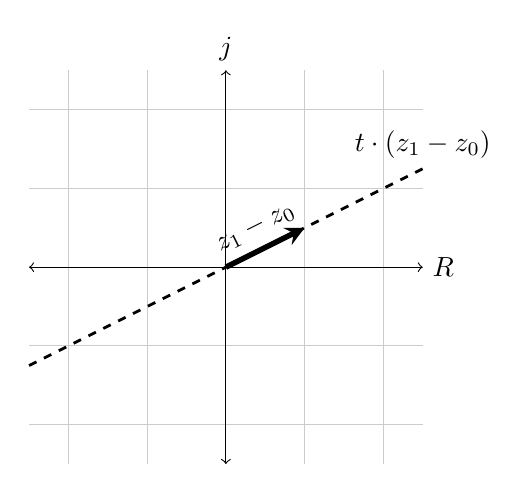
\begin{tikzpicture}
    \draw [thin,gray!40] (-2.5,-2.5) grid (2.5,2.5);
    \draw[<->] (-2.5,0)--(2.5,0) node[right] {$R$};
    \draw[<->] (0,-2.5)--(0,2.5) node[above]{$j$};
    \coordinate (a) at (1,1);
    \coordinate (b) at (3,2);
    \draw[line width=2pt,black,-stealth] (0,0)--(1,0.5) node[midway, above, sloped]{$z_1-z_0$};
    \draw[line width=1pt,black,dashed] (-2.5,-1.25)--(2.5,1.25) node[above]{$t\cdot(z_1-z_0)$};
\end{tikzpicture}
\caption*{Ecuación de la recta sin desplazar}
    \end{minipage}
    \begin{minipage}{0.4\textwidth}
        \centering
        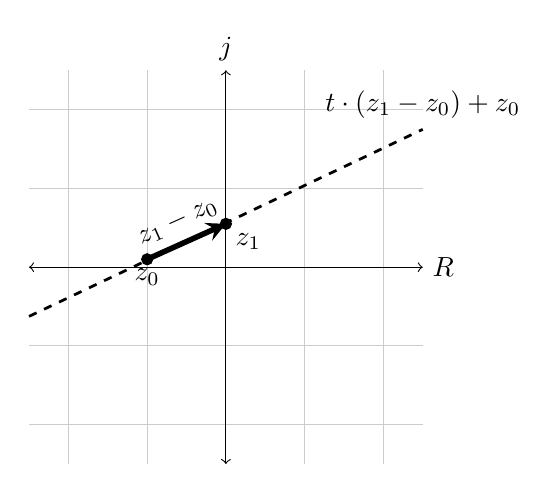
\begin{tikzpicture}
    \draw [thin,gray!40] (-2.5,-2.5) grid (2.5,2.5);
    \draw[<->] (-2.5,0)--(2.5,0) node[right] {$R$};
    \draw[<->] (0,-2.5)--(0,2.5) node[above]{$j$};
    \coordinate (a) at (-1,0.1);
    \coordinate (b) at (-0,0.55);
    \draw[fill=black] (a) circle(2pt) node[below]{$z_0$};
    \draw[fill=black] (b) circle(2pt) node[anchor=north west]{$z_1$};
    \draw[line width=2pt,black,-stealth] (a)--(b) node[midway, above, sloped]{$z_1-z_0$};
    \draw[line width=1pt,black,dashed] (-2.5,-0.625)--(2.5,1.75) node[above]{$t\cdot(z_1-z_0)+z_0$};
\end{tikzpicture}
\caption*{Ecuación de la recta desplazada}
    \end{minipage}
    \caption{Rectas definidas en coordenadas cartesianas}
    \label{fig:CartRectF}
\end{figure}
\unsubsubsection{Triangulo}
Ahora que están todas la herramientas necesarias presentadas construyamos un triangulo que tenga por vértices la coordenadas $\ a=(1,j0)$, $\ b=(3,j2)$, $\ c=(0.5+3j)$. Teniendo los puntos ya definidos y recordando la definición \ref{eq:RectaCarF}:
\begin{equation}
    \overline{z_{ab}}=t\cdot(z_b-z_a)+z_a \lrah\overline{z_{ab}}=t\cdot(2+2j)+1
    \begin{cases}
        t\therefore\overline{z_{ab}}=z_a\lrah t=0\\
        t\therefore\overline{z_{ab}}=z_b\lrah t=1\\
    \end{cases}
\end{equation}
Para la recta $\overline{z_{ab}}$, $t$ va a existir en el intervalo $0\leq t\leq1$ ya que cundo $t=1$ $\overline{z_{ab}}=z_b$ y cuando $t=0$ $\overline{z_{ab}}=z_a$. Se realiza el mismo analisis para las rectas $\overline{z_{bc}}$ y $\overline{z_{ca}}$
\begin{equation}
    \overline{z_{bc}}=t\cdot(z_c-z_b)+z_b \lrah\overline{z_{bc}}=t\cdot(-2.5+1j)+(3+j2)
    \begin{cases}
        0\leq t\leq1
    \end{cases}
\end{equation}
\begin{equation}
    \overline{z_{ca}}=t\cdot(z_a-z_c)+z_c \lrah\overline{z_{bc}}=t\cdot(0.5-3j)+(0.5+j3)
    \begin{cases}
         0\leq t\leq1
    \end{cases}
\end{equation}
\begin{figure}[H]
    \centering
    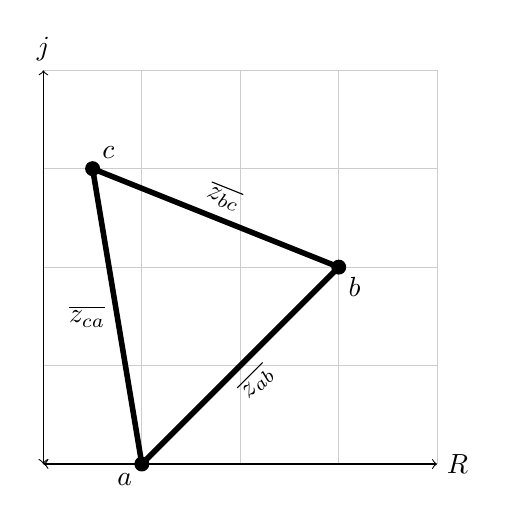
\begin{tikzpicture}[scale=1.25]
    \draw[thin,gray!40] (0,0) grid (4,4);
    \draw[<->] (0,0)--(4,0) node[right] {$R$};
    \draw[<->] (0,0)--(0,4) node[above]{$j$};
    \coordinate (a) at (1,0);
    \coordinate (b) at (3,2);
    \coordinate (c) at (0.5,3);
    
    \draw[fill=black] (a) circle(2pt) node[anchor=north east]{$a$};
    \draw[fill=black] (b) circle(2pt) node[anchor=north west]{$b$};
    \draw[fill=black] (c) circle(2pt) node[anchor=south west]{$c$};
    
    \draw[line width=2pt,black,-] (a)--(b) node[midway, below, sloped]{$\overline{z_{ab}}$};
    \draw[line width=2pt,black,-] (b)--(c) node[midway, above, sloped ]{$\overline{z_{bc}}$};
    \draw[line width=2pt,black,-] (c)--(a) node[midway, left]{$\overline{z_{ca}}$};
    
\end{tikzpicture}
\caption{Triangulo en el plano complejo con rectas parametrizadas}
    \label{fig:TrianCF}
\end{figure}

\unsubsection{Circunferencias, arcos, discos y segmentos de disco}
En el plano de 2 dimensiones una circunferencia es el lugar geométrico en el cual todos los punto pertenecientes al mismo tiene un distancia constante $r$ respecto a un punto $(a,b)$ de referencia llamado centro.
\begin{equation}\label{eq:DefCircR}
    \begin{aligned}
       (x-a)^2+(y-b)^2=r^2 \lrah \sqrt{(x-a^2+(y-b)^2}=&r \\
       |(x-a,y-b)|=&r
    \end{aligned}
\end{equation} 
Como podemos ver la ecuación \ref{eq:DefCircR} describe un modulo constante de valor $r$, esto en el plano complejo es fácil de definir, recordando las definiciones de la forma polar\ref{eq:defPol} y exponencial\ref{eq:defExp} dejando el modulo $r$ como una constante y dejamos el argumento como un  parámetro. Recordando que el argumento de un numero complejo esta definido como $-\pi<\theta\leq\pi$:
\begin{equation}\label{eq:ParamcircF}
    z=re^{j\theta}+z_0 \llrah\ z=r[\cos{(\theta)}+j\sen{(\theta)}]+z_0
\end{equation}
\begin{equation}
    re^{j\theta}
    \begin{cases}
        r=\kappa\\
        -\pi<\theta\leq\pi
    \end{cases}
\end{equation}
\begin{figure}[H]
    \centering
    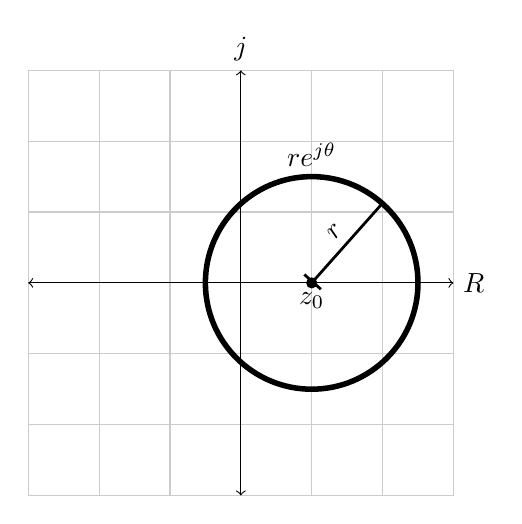
\begin{tikzpicture} [scale=0.9]
    \draw[thin,gray!40] (-3,-3) grid (3,3);
    \draw[<->] (-3,0)--(3,0) node[right] {$R$};
    \draw[<->] (0,-3)--(0,3) node[above]{$j$};
    \draw[line width=2pt] (1,0) circle(1.5);
    \draw[] (1,1.5) node[above]{$re^{j\theta}$};
    \draw[fill=black] (1,0) circle(2pt) node[below]{$z_0$};
    \draw[line width=1pt,black,|-|] (1,0)--(2,1.125) node[midway,above,sloped]{$r$};
\end{tikzpicture}
\caption{Circunferencia en el plano complejo de centro $z_0$}
    \label{fig:CircCF}
\end{figure}
Restringiendo el intervalo en el que existe el argumento podremos crear un arco. Un ejemplo seria $-\frac{\pi}{4}\leq\theta\leq\frac{\pi}{4}$:
\begin{equation}
    re^{j\theta}+z_0
    \begin{cases}
        r=\kappa\\
        -\frac{\pi}{4}\leq\theta\leq\frac{\pi}{4}
    \end{cases}
\end{equation}
\begin{figure}[H]
    \centering
    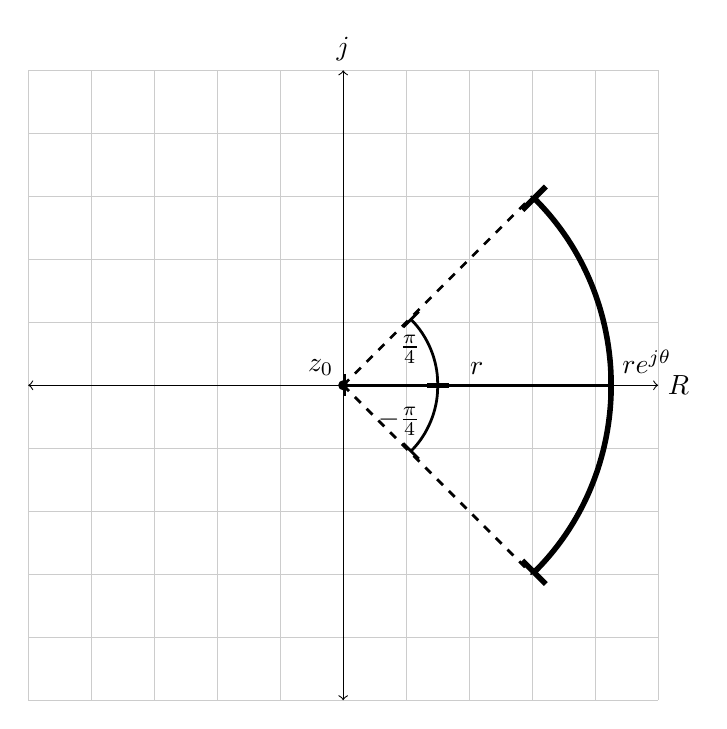
\begin{tikzpicture}[scale=0.8]
    \draw[thin,gray!40] (-5,-5) grid (5,5);
    \draw[<->] (-5,0)--(5,0) node[right] {$R$};
    \draw[<->] (0,-5)--(0,5) node[above]{$j$};
    \draw[line width=2pt,black,|-|] (3,-3) arc (-45:45:4.2426) node [midway,anchor=south west]{$re^{j\theta}$};
    \draw[line width=1pt,black,|-|] (1.5,0) arc (0:45:1.5) node [midway, left]{$\frac{\pi}{4}$};
    \draw[line width=1pt,black,|-|] (1.5,0) arc (0:-45:1.5) node [midway, left]{$-\frac{\pi}{4}$};
    \draw[fill=black] (0,0) circle(2pt) node[anchor=south east]{$z_0$};
    \draw[line width=1pt,black,dashed] (0,0)--(3,3);
    \draw[line width=1pt,black,dashed] (0,0)--(3,-3);
    \draw[line width=1pt,black,|-|] (0,0)--(4.2426,0) node[midway,above,sloped]{$r$};

  
\end{tikzpicture}
\caption{Arco en el plano complejo de centro $z_0$}
    \label{fig:ArcCF}
\end{figure}

Ahora si además de variar el argumento sin restringirlo y asociamos a $r$ con intervalo del tipo $r_0\leq r\leq r_1$ generaremos un disco de radio interior $r_0$ y radio exterior $r_1$:
\begin{equation}
    re^{j\theta}+z_0
    \begin{cases}
        r_0\leq r\leq r_1\\
        -\pi<\theta\leq\pi
    \end{cases}
\end{equation}
\begin{figure}[H]
    \centering
    \begin{tikzpicture}
    \draw[thin,gray!40] (-4,-4) grid (4,4);
    \draw[<->] (-4,0)--(4,0) node[right] {$R$};
    \draw[<->] (0,-4)--(0,4) node[above]{$j$};
    \fill[fill=mlgb, fill opacity=0.6,even odd rule] (0,0) circle (3) (0,0) circle (1);
    \draw[fill=black] (0,0) circle(2pt) node[anchor=north east]{$z_0$};
    \draw[line width=1pt,|-|] (0,0) -- (0.707,0.707) node[midway,above,sloped]{$r_0$};
    \draw[line width=1pt,|-|] (0,0) -- (-2.1213,2.1213) node[midway,above,sloped]{$r_1$};
    \draw [black,line width=2pt](0, 0) circle (1);
    \draw [black,line width=2pt](0, 0) circle (3);
\end{tikzpicture}
\caption{Disco en el plano complejo}
    \label{fig:DiscoCF}
\end{figure}
Conociendo todo esto y además recordando la definición de rectas en el plano complejo \ref{eq:RectaCarF} se podrá definir un segmento de disco. Planteando un ejemplo en el cual los vértices del segmento sean $a=(1,j0.5)$, $\ b=(3+j0.5)$, $\ c=(1.521+j3.512)$ y $\ d=(0.559+j1.291)$. Como vemos nuestro segmento estará conformado por una linea horizontal $\ \overline{ab}$, dos arcos $\ \vec{bc}$, $\ \Vec{da}$ y una recta $\overline{z_{cd}}$.
\begin{equation}
    \overline{ab}=(t+j\kappa)\lrah
    \begin{cases}
        \kappa=0.5\\
        1\leq t\leq3
    \end{cases}
\end{equation}
\begin{equation}
    \overline{z_{cd}}=t\cdot(z_c-z_d)+z_d \lrah\overline{z_{cd}}=t\cdot(0.962+2.221j)+(0.559+j1.291)
    \begin{cases}
         0\leq t\leq1
    \end{cases}
\end{equation}
El arco $\vec{bc}$ debe tener necesariamente el mismo modulo que los puntos por donde pasa y el argumento debe variar en un intervalo desde el argumento del punto inicial hasta el argumento del punto final.
\begin{equation}
    \vec{bc}=re^{j\theta}
    \begin{cases}
        \tan^{-1}{\frac{\Imag{b}}{\Real{b}}}\leq\theta\leq\tan^{-1}{\frac{\Imag{c}}{\Real{z_c}}}\lrah0.052\pi\leq\theta\leq0.367\pi\\
        \\
        r=|c|=|b|=3.04
    \end{cases}
\end{equation}
\begin{equation}
    \vec{da}=re^{j\theta}
    \begin{cases}
        \tan^{-1}{\frac{\Imag{a}}{\Real{a}}}\leq\theta\leq\tan^{-1}{\frac{\Imag{d}}{\Real{d}}}\lrah0.148\pi\leq\theta\leq0.367\pi\\
        \\
        r=|d|=|a|=1.18
    \end{cases}
\end{equation}
\begin{figure}[H]
    \centering
    \begin{tikzpicture}[scale=1.5]
    \draw[thin,gray!40] (0,0) grid (4,4);
    \draw[<->] (0,0)--(4,0) node[right] {$R$};
    \draw[<->] (0,0)--(0,4) node[above]{$j$};
    \coordinate (a) at (1,0.5);
    \coordinate (b) at (3,0.5);
    \coordinate (c) at (1.521,2.634);
    \coordinate (d) at (0.559,1.022);
    
    \fill[fill=mlgb,opacity=0.6,even odd rule](a)--(b) arc (9.4623:60:3.0414)--(0.54,1.022) arc (60:26.56505:0.8)--(a) ;
    
    \draw[fill=black] (a) circle(2pt) node[anchor=north]{$a$};
    \draw[fill=black] (b) circle(2pt) node[anchor=north]{$b$};
    \draw[fill=black] (c) circle(2pt) node[anchor=south]{$c$};
    \draw[fill=black] (d) circle(2pt) node[anchor=east]{$d$};
    
    \draw[line width=2pt,black,-] (a)--(b) node[midway, below]{$\overline{ab}$};
    \draw[line width=2pt,black,-] (b) arc (9.4623:60:3.0414) node [midway,anchor=south west]{$\Vec{bc}$};
    \draw[line width=2pt,black,-] (c)--(d) node[midway, above,sloped]{$\overline{cd}$};
    \draw[line width=2pt,black,-] (a) arc (26.56505:60:1.18) node [midway,anchor=north east]{$\Vec{da}$};

    
    
\end{tikzpicture}
\caption{Segmento de disco en el plano complejo con lineas parametrizadas}
    \label{fig:SegDiscCF}
\end{figure}

Podemos plantear otro ejemplo con los puntos a $a=(1,j)$, $b=(2,j2)$, $c=(-1,j)$ y $d=(-2,2j)$ como vemos el segmento del disco estará conformado por las rectas $\overline{ab}$, $\overline{cd}$ y los arcos $\vec{bc}$, $\vec{da}$:
\begin{equation}
    \begin{aligned}
        \overline{ab}&=t\cdot(z_b-z_a)+z_a
        \begin{cases}
        \overline{ab}=t\cdot(1+j)+(1+j) \llrah\ re^{j\frac{\pi}{4}}\\
            0\leq t\leq 1 \llrah\ 1\leq r\leq 2
        \end{cases}\\
        \\
        \overline{cd}&=t\cdot(z_d-z_c)+z_c 
        \begin{cases}
        \overline{cd}=t\cdot(-1+j)+(-1+j) \llrah\ re^{j\frac{4\pi}{3}}\\
            0\leq t\leq 1 \llrah\ 1\leq r\leq 2
        \end{cases}\\
    \end{aligned}
\end{equation}
\begin{equation}
    \begin{aligned}
     \vec{bd}&=re^{j\theta}
    \begin{cases}
       \frac{\pi}{4}\leq\theta\leq\frac{4\pi}{3}\\
        \\
        r=|c|=|b|=2
    \end{cases}\\
     \vec{ca}&=re^{j\theta}
    \begin{cases}
       \frac{\pi}{4}\leq\theta\leq\frac{4\pi}{3}\\
        \\
        r=|d|=|a|=1
    \end{cases}
    \end{aligned}
\end{equation}
\begin{figure}[H]
    \centering
    \begin{tikzpicture}
    \draw[thin,gray!40] (-5,0) grid (5,6);
    \draw[<->] (-5,0)--(5,0) node[right] {$R$};
    \draw[<->] (0,0)--(0,6) node[above]{$j$};
    \coordinate (a) at (1,1);
    \coordinate (b) at (3,3);
    \coordinate (c) at (-1,1);
    \coordinate (d) at (-3,3);
    \fill[fill=mlgb,opacity=0.6,even odd rule](a)--(b) arc (45:135:4.2426)--(c)  arc (135:45:1.4142)--(a) ;
    
    \draw[fill=black] (a) circle(2pt) node[anchor=north west]{$a$};
    \draw[fill=black] (b) circle(2pt) node[anchor=south west]{$b$};
    \draw[fill=black] (c) circle(2pt) node[anchor=north east]{$c$};
    \draw[fill=black] (d) circle(2pt) node[anchor=south east]{$d$};
    
    \draw[line width=2pt,black,-] (a)--(b) node[midway, right]{$\overline{ab}$};
    \draw[line width=2pt,black,-] (c)--(d) node[midway, left]{$\overline{cd}$};
    \draw[line width=2pt,black,-] (b) arc (45:135:4.2426) node [midway,above]{$\Vec{bc}$};
    \draw[line width=2pt,black,-] (a) arc (45:135:1.4142) node [midway,below]{$\Vec{da}$};
    
\end{tikzpicture}
\caption{Segmento de disco en el plano complejo con lineas parametrizadas}
    \label{fig:SegDiscCF2}
\end{figure}

\unsection{Funciones complejas}
Un función compleja rige el comportamiento de el plano complejo en su totalidad y transforma números complejos a números complejos. Se podría decir que una función compleja toma el plano complejo $z$ y lo transforma en otro plano complejo $w$. 
Una función compleja se define de la siguiente manera:
\begin{equation}
    f(z)=w
\end{equation}
\begin{figure}[H]
\centering
    \begin{minipage}{0.4\textwidth}
    \centering
       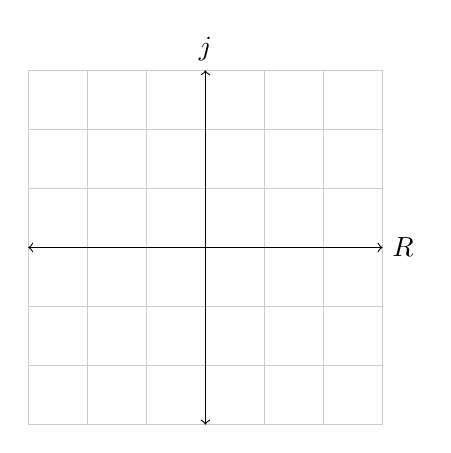
\begin{tikzpicture}[scale= 0.75]
        \draw[thin,gray!40] (-3,-3) grid (3,3);
        \draw[<->] (-3,0)--(3,0) node[right] {$R$};
        \draw[<->] (0,-3)--(0,3) node[above]{$j$};
\end{tikzpicture}
\caption*{Plano complejo $z$}
    \label{fig:PlanoCF1}
    \end{minipage}%
    \begin{minipage}[t]{0.2\textwidth}
        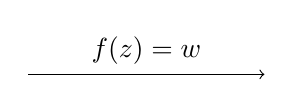
\begin{tikzpicture}
        \centering
            \draw[->] (0,0)--(3,0) node[midway, above] {$f(z)=w$};
        \end{tikzpicture} 
    \end{minipage}%
   \begin{minipage}{0.4\textwidth}
    \centering
       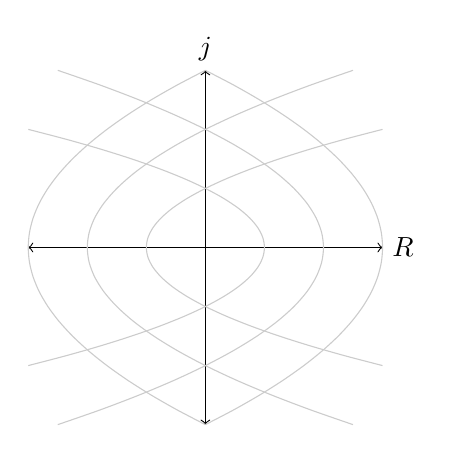
\begin{tikzpicture}[scale= 0.75]
        \draw[<->] (-3,0)--(3,0) node[right] {$R$};
        \draw[<->] (0,-3)--(0,3) node[above]{$j$};
        \draw[rotate=90,thin,gray!40]   plot[smooth,domain=-2:2] (\x, {((\x)^2)-1});
        \draw[rotate=90,thin,gray!40]   plot[smooth,domain=-3:3] (\x, {((\x)^2)/2-2});
        \draw[rotate=90,thin,gray!40]   plot[smooth,domain=-3:3] (\x, {((\x)^2)/3-3});
        \draw[rotate=-90,thin,gray!40]   plot[smooth,domain=-2:2] (\x, {((\x)^2)-1});
        \draw[rotate=-90,thin,gray!40]   plot[smooth,domain=-3:3] (\x, {((\x)^2)/2-2});
        \draw[rotate=-90,thin,gray!40]   plot[smooth,domain=-3:3] (\x, {((\x)^2)/3-3});
\end{tikzpicture}
\caption*{Plano complejo $w$}
    \label{fig:PlanoCF2}
    \end{minipage}%
    \caption{}
    \label{fig:CompPLF}
\end{figure}
La convención es que la variable independiente se la llame $\ z=x+jy$ y la dependiente $\ w=u+jv$. Como en el caso de las ecuaciones una función compleja también se puede sub dividir en 2 partes, una que rija la parte real y otra que rija la parte imaginaria.Para visualizar como funcionan las funciones complejas se utiliza el mapeo de curvas parametrizadas como herramienta.

El concepto del mapeo es tomar una curva y ver como seria transformada en el plano $w$ aplicándole la función únicamente a la curva y graficarlo sobre el plano $z$, como si estuviéramos tomando una muestra del plano complejo $w$.
\unsubsection{Desplazamiento}
Un desplazamiento en el plano complejo se define con la forma de:
\begin{equation}\label{eq:defDespF}
    w=z+z_0
\end{equation}
Siendo $z_0$ un numero complejo, esta función desplaza todo los puntos del plano $z$ en $z_0$. Viendo como se modifica la parte real y parte imaginaria queda implicito el desplazamiento:
\begin{equation}
    w=z+z_0\lrah(u+jv)=(x+jy)+(x_0+jy_0)
    \begin{cases}
        u=x+x_0\\
        v=y+y_0
    \end{cases}
\end{equation}
Para ver gráficamente como se mapea el plano $z$ en el plano $w$, plantemos un rectángulo en el plano $z$ y le apliquemos la función desplazamiento:
\begin{equation}\label{eq:EjemDespF}
    w=z+z_0\lrah w=z+(1+j)    
\end{equation}
por ejemplo. 

El rectángulo $S$ en el plano $z$ sera  el del ejemplo de la figura \ref{fig:RectF}. Recordemos que los puntos que define al rectángulos en el plano $z$ son $\ a=(1+j)$, $\ b=(3+j)$, $\ c=(3+j2)$ y $d\ =(1+2j)$ entonces en el plano $z$, el rectángulo, esta descripto por las ecuaciones:
\begin{equation}
    \begin{aligned}
        \overline{ab}&=(t+j);\  1\leq t\leq3;\\
        \overline{cd}&=(t+j2);\  1\leq t\leq3;\\
        \overline{bc}&=(3+jt);\  1\leq t\leq2;\\
        \overline{da}&=(1+jt);\  1\leq t\leq2;
    \end{aligned}
\end{equation}
Aplicando la función desplazamiento\ref{eq:EjemDespF} a las ecuaciones:
\begin{equation}
    \begin{aligned}
         f_{(\overline{ab})}&=(t+j)+(1+j)  \lrah\ \overline{ab}'=(t+1)+j2\ ;\  1\leq t\leq3;\\
         f_{(\overline{cd})}&=(t+j2)+(1+j) \lrah \overline{cd}'=(t+1)+j3\ ;\  1\leq t\leq3;\\
         f_{(\overline{bc})}&=(3+jt)+(1+j) \lrah \overline{bc}'=4+j(t+1)\ ;\  1\leq t\leq2;\\
         f_{(\overline{da})}&=(1+jt)+(1+j) \lrah \overline{da}'=2+j(t+1)\ ;\  1\leq t\leq2;
    \end{aligned}
\end{equation}
Haciendo un cambio de variable $t'=(t+1)$ quedarían definidos como:
\begin{equation}
    \begin{aligned}
        &\overline{ab}'=t'+j2\ ;\  2\leq t'\leq4;\\
        &\overline{cd}'=t'+j3\ ;\  2\leq t'\leq4;\\
        &\overline{bc}'=4+jt'\ ;\  2\leq t'\leq3;\\
        &\overline{da}'=2+jt'\ ;\  2\leq t'\leq3;
    \end{aligned}
\end{equation}
\begin{figure}[H]
    \centering
    \begin{minipage}{0.39\textwidth}
    \centering
        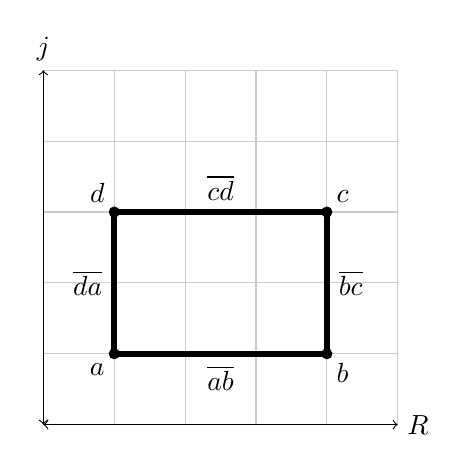
\begin{tikzpicture}[scale=0.9]
    \draw[thin,gray!40] (0,0) grid (5,5);
    \draw[<->] (0,0)--(5,0) node[right] {$R$};
    \draw[<->] (0,0)--(0,5) node[above]{$j$};
    \coordinate (1) at (1,1);
    \coordinate (2) at (4,1);
    \coordinate (3) at (4,3);
    \coordinate (4) at (1,3);
    
    \draw[fill=black] (1) circle(2pt) node[anchor=north east]{$a$};
    \draw[fill=black] (2) circle(2pt) node[anchor=north west]{$b$};
    \draw[fill=black] (3) circle(2pt) node[anchor=south west]{$c$};
    \draw[fill=black] (4) circle(2pt) node[anchor=south east]{$d$};
    
    \draw[line width=2pt,black,-] (1)--(2) node[midway, below]{$\overline{ab}$};
    \draw[line width=2pt,black,-] (2)--(3) node[midway, right]{$\overline{bc}$};
    \draw[line width=2pt,black,-] (3)--(4) node[midway, above]{$\overline{cd}$};
    \draw[line width=2pt,black,-] (4)--(1) node[midway, left]{$\overline{da}$};
    
\end{tikzpicture}
\caption*{Rectángulo $s$}

    \end{minipage}
    \begin{minipage}[t]{0.2\textwidth}
    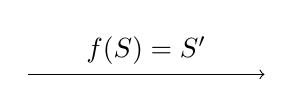
\begin{tikzpicture}
        \centering
            \draw[->] (0,0)--(3,0) node[midway, above] {$f(S)=S'$};
        \end{tikzpicture} 
    \end{minipage}
    \begin{minipage}{0.39\textwidth}
    \centering
        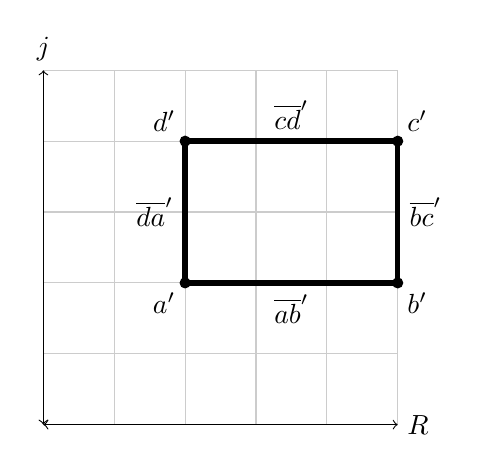
\begin{tikzpicture}[scale=0.9]
    \draw[thin,gray!40] (0,0) grid (5,5);
    \draw[<->] (0,0)--(5,0) node[right] {$R$};
    \draw[<->] (0,0)--(0,5) node[above]{$j$};
    \coordinate (a) at (2,2);
    \coordinate (b) at (5,2);
    \coordinate (c) at (5,4);
    \coordinate (d) at (2,4);
    
    \draw[fill=black] (a) circle(2pt) node[anchor=north east]{$a'$};
    \draw[fill=black] (b) circle(2pt) node[anchor=north west]{$b'$};
    \draw[fill=black] (c) circle(2pt) node[anchor=south west]{$c'$};
    \draw[fill=black] (d) circle(2pt) node[anchor=south east]{$d'$};
    
    \draw[line width=2pt,black,-] (a)--(b) node[midway, below]{$\overline{ab}'$};
    \draw[line width=2pt,black,-] (b)--(c) node[midway, right]{$\overline{bc}'$};
    \draw[line width=2pt,black,-] (c)--(d) node[midway, above]{$\overline{cd}'$};
    \draw[line width=2pt,black,-] (d)--(a) node[midway, left]{$\overline{da}'$};
    
\end{tikzpicture}
\caption*{Mapeo de el rectangulo $S$}
    \end{minipage}
    \caption{}
\end{figure}
Podemos graficar el plano $w$ en el plano $z$ para denotar como el la función desplazamiento mueve el plano complejo.
\begin{figure}[H]
    \centering
    \begin{tikzpicture}[scale=1.5]
    \draw[thin,gray!40] (0,0) grid (5,5);
    \draw[mlgb,line width=1pt, ->] (0,0)--(5,0) node[right] {$R$};
    \draw[mlgb,line width=1pt, ->] (0,0)--(0,5) node[above]{$j$};
    \draw[line width=1pt, <->] (0,1)--(5,1) node[right] {$R'$};
    \draw[line width=1pt, <->] (1,0)--(1,5) node[above]{$j'$};
    \coordinate (1) at (1,1);
    \coordinate (2) at (4,1);
    \coordinate (3) at (4,3);
    \coordinate (4) at (1,3);
    \coordinate (a) at (2,2);
    \coordinate (b) at (5,2);
    \coordinate (c) at (5,4);
    \coordinate (d) at (2,4);
    
    \draw[fill=black] (1) circle(2pt) node[anchor=south east]{$z_0$} node[mlgb,anchor=north west]{$a$};
    \draw[mlgb,fill=mlgb] (2) circle(1pt) node[anchor=north west]{$b$};
    \draw[mlgb,fill=mlgb] (3) circle(1pt) node[anchor=south east]{$c$};
    \draw[mlgb,fill=mlgb] (4) circle(1pt) node[anchor=south east]{$d$};
    
    \draw[fill=black] (a) circle(2pt) node[anchor=north west]{$a'$};
    \draw[fill=black] (b) circle(2pt) node[anchor=north]{$b'$};
    \draw[fill=black] (c) circle(2pt) node[anchor=south east]{$c'$};
    \draw[fill=black] (d) circle(2pt) node[anchor=south east]{$d'$};
    
    \draw[line width=1pt,mlgb,dashed] (1)--(2) node[midway, below]{$\overline{ab}$};
    \draw[line width=1pt,mlgb,-] (2)--(3) node[midway, right]{$\overline{bc}$};
    \draw[line width=1pt,mlgb,-] (3)--(4) node[midway, above]{$\overline{cd}$};
    \draw[line width=1pt,mlgb,dashed] (4)--(1) node[midway, left]{$\overline{da}$};
    
    \draw[line width=2pt,black,-] (a)--(b) node[midway, below]{$\overline{ab}'$};
    \draw[line width=2pt,black,-] (b)--(c) node[midway, right]{$\overline{bc}'$};
    \draw[line width=2pt,black,-] (c)--(d) node[midway, above]{$\overline{cd}'$};
    \draw[line width=2pt,black,-] (d)--(a) node[midway, left]{$\overline{da}'$};

    \draw[line width=2pt,black, -stealth] (0,0)--(1) node[midway, left]{};
    \draw[line width=1pt,black,dotted] (1)--(a) node[midway, left]{};
    \draw[line width=1pt,black,dotted] (3)--(c) node[midway, left]{};
    \draw[line width=1pt,black,dotted] (2)--(b) node[midway, left]{};
    \draw[line width=1pt,black,dotted] (4)--(d) node[midway, left]{};
    
\end{tikzpicture}
\caption{Plano $w$ graficado sobre el plano $z$ siendo $f_z$ un desplazamiento}
    \label{fig:DespZWF}
\end{figure}
Como se pude interpretar en la figura \ref{fig:DespZWF} cualquier curva parametrizada ahora estará desplazada en $z_0$, recordando la parametrizaciones las curvas dadas en \ref{eq:ParamcircF} y \ref{eq:RectaCarF}, rectas y circunferencias se mapean en:
\begin{equation}
    f_{(z)}=z+z_0
    \begin{cases}
        f_{(z)}=[t\cdot(z_a-z_b)+z_c]+z_0 \lrah f_{(z)}=t\cdot(z_a-z_b)+(z_c+z_0)\\
        f_{(z)}=[re^{j\theta}+z_c]+z_0 \lrah  f_{(z)}=re^{j\theta}+(z_c+z_0)
    \end{cases}
\end{equation}
Entonces el desplazamiento modifica los centros de las circunferencia-arcos y la ordenada al origen de las rectas.

\unsubsection{Escalado}
La función escaldo se define como:
\begin{equation}
    w=\lambda\cdot z
\end{equation}
$\lambda$ siendo un numero real. 
Planteando un numero complejo de la forma $z=re^{j\theta}$ y $z=(a+jb)$ podemos ver que la función escalado se comporta como:
\begin{equation}
    w=\lambda z
    \begin{cases}
        w=\lambda\cdot (re^{j\theta})\lrah w=(\lambda r)e^{j\theta}\\
        w=\lambda\cdot(a+jb)\lrah w=(\lambda a)+j(\lambda b) 
    \end{cases}
\end{equation}
Recordando las propiedades del operador $||$, vemos que la función escalado no modifico el argumento del numero complejo solo escala el modulo por un factor $\lambda$. Separando la expresión en su parte real e imaginaria se ve que ambas partes están escaladas por el mismo factor:
\begin{equation}
    w=\lambda z\lrah (u+jv)=\lambda(x+jy)
    \begin{cases}
        u=\lambda x
        v=\lambda y
    \end{cases}
\end{equation}
Plantemos un disco, un segmento de recta y una recta para apreciar como se modifican el plano $w$ con respecto al $z$:
\begin{equation}
    \begin{aligned}
        \vec{a}=&re^{j\theta}+z_c\lrah 1e^{j\theta}+(-1+j)\\
         z_0=&t(z_a-z_b)+z_b\lrah t(1+j)+2\llrah\ te^{j\frac{\pi}{4}}+2\begin{cases}
            1\leq t\leq\ 2
    \end{cases}\\
        z_1=&t(z_c-z_d)+z_b\lrah t(1.376+j)\llrah\ te^{j\frac{\pi}{5}}\begin{cases}
            -\infty\leq t\leq\infty
    \end{cases}
    \end{aligned}
\end{equation}
Aplicando les un escalado de $\lambda=2$ las expresiones quedarían como:
\begin{equation}
    \begin{aligned}
        f_{(\Vec{a})}=&\lambda (2e^{j\theta}+(-1-j))\lrah 4e^{j\theta}+(-2-j2)\\
        f_{(z_0)}=&\lambda(t(1+j)+2)\lrah w_0=2t(1+j)+4\llrah\ 2te^{j\frac{\pi}{4}}+4\begin{cases}
            1\leq t\leq\ 2
    \end{cases}\\
        f_{(z_1)}=&\lambda(t(1.376+j)) \lrah w_1=2t(1.376+j)\llrah\ 2te^{j\frac{\pi}{5}}\begin{cases}
            -\infty\leq t\leq\infty
    \end{cases}
    \end{aligned}
\end{equation}
Haciendo un cambio de variable $t'=2t$, las expresiones del segmento de recta y la recta quedarían de la siguiente manera:
\begin{equation}
    \begin{aligned}
        w_0=&2t(1+j)+4\begin{cases}
            1\leq t\leq\ 3
    \end{cases}\lrah w_0=t'(1+j)+4\begin{cases}
            2\leq t'\leq\ 4
    \end{cases}\\
        w_1=& 2t(1.376+j)\begin{cases}
            -\infty\leq t\leq\infty
        \end{cases}\lrah w_1=t'(1.376+j)\begin{cases}
            -\infty\leq t'\leq\infty
        \end{cases}
    \end{aligned}
\end{equation}
El escalamiento modifico la ordenada al origen de la recta $z_0$ y el centro de la circunferencia $\Vec{a}$, multiplicando ambos puntos por $\lambda$.Entonces podemos decir que los objetos mapeados que tengan por centro el punto $(0,j0)$ en el plano $z$ no se veran desplazados y su centro sera el mismo. Si los objetos sufren de un desplazamiento en $z_c$ en el plano $z$, se verán desplazados $\lambda z_c$ en el plano $w$.

También vemos el escalamiento modifica la extensión de los intervalos acotados, en este ejemplo pasamos de un intervalo de modulo 1 a un intervalo de modulo 2. Otra forma de interpretarlo es que el escalado, en el caso de las rectas aumenta el tamaño del modulo del vector $(z_0-z_1)$ que describe la recta, en vez de modificar la longitud de los intervalos del parámetro $t$. Recordemos la definición de una recta que pasa por 2 puntos \ref{eq:RectaCarF}:
\begin{equation}
    \begin{aligned}
        f_{(z_0)}=&\lambda(t(1+j)+2)\lrah w_0=t(2+j2)+4\begin{cases}
            1\leq t\leq\ 2
    \end{cases}\\
        f_{(z_1)}=&\lambda(t(1.376+j)) \lrah w_1=t(2.752+j2) \begin{cases}
            -\infty\leq t\leq\infty
    \end{cases}
    \end{aligned}
\end{equation}
\begin{figure}[H]
    \centering
    \begin{minipage}{0.39\textwidth}
         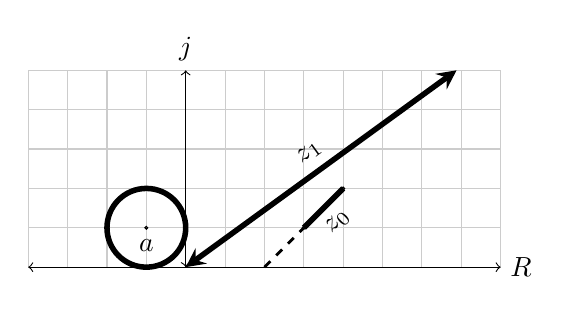
\begin{tikzpicture}[scale=0.5]
    \draw [thin,gray!40] (-4,0) grid (8,5);
    \draw[<->] (-4,0)--(8,0) node[right] {$R$};
    \draw[<->] (0,0)--(0,5) node[above]{$j$};
    \coordinate (a) at (-1,1);
    \coordinate (b) at (3,1);
    \coordinate (c) at (4,2);
    \coordinate (d) at (-5,-3.634);
    \coordinate (e) at (6.88,5);
    \coordinate (f) at (2,0);
    
    \draw[line width=2pt,black] (a) circle(1) node[anchor=north]{$\Vec{a}$};
    \draw[black] (a) circle(1pt) node[anchor=south]{};
    \draw[black] (b) circle(1pt) node[anchor=south]{};
    \draw[black] (c) circle(1pt) node[anchor=south]{};
    \draw[line width=2pt,black,-] (b)--(c) node[midway, below, sloped]{$z_0$};
    \draw[line width=2pt,black,stealth-stealth] (0,0)--(e) node[midway,above,sloped]{$z_1$};
    \draw[line width=1pt,black,dashed] (f)--(b) node[midway, above, sloped]{};
\end{tikzpicture}
\caption*{Figuras sin escalar}
    \end{minipage}
     \begin{minipage}{0.2\textwidth}
    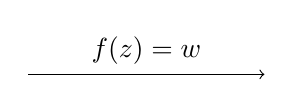
\begin{tikzpicture}
        \centering
            \draw[->] (0,0)--(3,0) node[midway, above] {$f(z)=w$};
        \end{tikzpicture} 
    \end{minipage}
    \begin{minipage}{0.39\textwidth}
         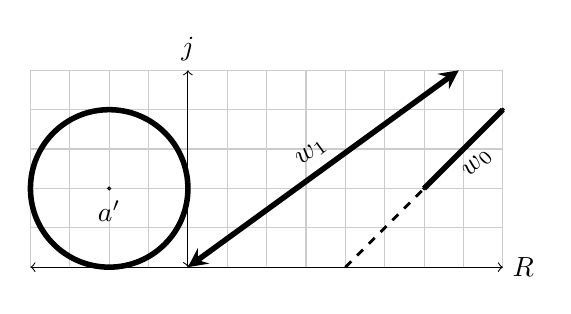
\begin{tikzpicture}[scale=0.5]
    \draw [thin,gray!40] (-4,0) grid (8,5);
    \draw[<->] (-4,0)--(8,0) node[right] {$R$};
    \draw[<->] (0,0)--(0,5) node[above]{$j$};
    \coordinate (a) at (-2,2);
    \coordinate (b) at (6,2);
    \coordinate (c) at (8,4);
    \coordinate (d) at (-5,-3.634);
    \coordinate (e) at (6.88,5);
    \coordinate (f) at (4,0);
    
    \draw[line width=2pt,black] (a) circle(2) node[anchor=north]{$\Vec{a'}$};
    \draw[black] (a) circle(1pt) node[anchor=south]{};
    \draw[black] (b) circle(1pt) node[anchor=south]{};
    \draw[black] (c) circle(1pt) node[anchor=south]{};
    \draw[line width=2pt,black,-] (b)--(c) node[midway, below, sloped]{$w_0$};
    \draw[line width=2pt,black,stealth-stealth] (0,0)--(e) node[midway,above,sloped]{$w_1$};
    \draw[line width=1pt,black,dashed] (f)--(b) node[midway, above, sloped]{};
\end{tikzpicture}
\caption*{Figuras escaladas}
    \end{minipage}
    \caption{}
\end{figure}
En el caso de la recta $z_1$ el escalado no tiene prácticamente ningún efecto ya que no sufre de desplazamientos y los vectores que describe la recta y su transformación, $(1.376+j)$ y $(2.752+j2)$, son múltiplos entre si, además la recta esta definida hasta el infinito, el único parámetro relevante, entonces, es el ángulo con respecto al eje $R$ y para ambos vectores es el mismo. En términos de tendencia técnicamente la recta transformada $w_1$ tiende mas rápido al infinito ya que la derivada con respecto al parámetro $t$ es el doble de la recta sin transformar.

Todos los cambios sufridos por las curvas parametrizadas que usamos de ejemplo se pueden ver intuitivamente si pensamos en el escalado como una dilatación del plano complejo $z$.
\begin{figure}[H]
    \centering
    \begin{tikzpicture}[scale=0.8]
    
    \draw [thin,mlgb] (-8,-3) grid (8,8);
    \draw [step=2.0,line width=0.5pt,gray] (-8,-3) grid (8,8);
    \draw[mlgb,<->] (-8,0)--(8,0) node[anchor= north west] {$R$};
    \draw[mlgb,<->] (0,-3)--(0,8) node[anchor=south east]{$j$};
    \draw[<->] (-8,0)--(8,0) node[anchor=south west] {$R'$};
    \draw[<->] (0,-3)--(0,8) node[anchor=south west]{$j'$};

    \coordinate (1) at (-1,1);
    \coordinate (2) at (3,1);
    \coordinate (3) at (4,2);
    \coordinate (4) at (-5,-3.634);
    \coordinate (5) at (8, 5.814);
    \coordinate (6) at (2,0);
    \coordinate (7) at (3,2);
    \coordinate (8) at (4,1);
    
    \coordinate (a) at (-2,2);
    \coordinate (b) at (6,2);
    \coordinate (c) at (8,4);
    \coordinate (d) at (-5,-3.634);
    \coordinate (e) at (8, 5.814);
    \coordinate (f) at (4,0);
    \coordinate (g) at (6,4);
    \coordinate (h) at (8,2);

    \draw[line width=1pt,gray,dotted] (-1,2)--(-2,4) ;
    \draw[line width=1pt,gray,dotted] (-2,1)--(-4,2) ;
    \draw[line width=1pt,gray,dotted] (-1.707,1.707)--(-3.414,3.414) ;
    \draw[line width=1pt,gray,dotted] (-0.293,0.293)--(-0.586,0.586) ;
    \draw[line width=1pt,gray,dotted] (-1.707,0.293)--(-3.414,0.586) ;
    \draw[line width=1pt,gray,dotted] (-0.293,1.707)--(-0.586,3.414) ;
    \draw[line width=1pt,gray,dotted] (2)--(b) ;
    \draw[line width=1pt,gray,dotted] (3)--(c) ;
    \draw[line width=1pt,gray,dotted] (7)--(g) ;
    \draw[line width=1pt,gray,dotted] (8)--(h) ;
    \draw[line width=1pt,black,dashed] (2)--(7);
    \draw[line width=1pt,black,dashed] (7)--(3);
    \draw[line width=1pt,black,dashed] (3)--(8);
    \draw[line width=1pt,black,dashed] (8)--(2);
    \draw[line width=1pt,black,-] (b)--(g);
    \draw[line width=1pt,black,-] (g)--(c);
    \draw[line width=1pt,black,-] (c)--(h);
    \draw[line width=1pt,black,-] (h)--(b);

    
    \draw[line width=1pt,mlgb] (1) circle(1) node[anchor=north]{$\Vec{a}$};
    \draw[mlgb] (1) circle(1pt) node[anchor=south]{};
    \draw[mlgb] (2) circle(1pt) node[anchor=south]{};
    \draw[mlgb] (3) circle(1pt) node[anchor=south]{};
    \draw[line width=1pt,mlgb,-] (2)--(3) node[midway, above, sloped]{$z_0$};
   
    
    \draw[line width=2pt,black] (a) circle(2) node[anchor=north]{$\Vec{a'}$};
    \draw[black] (a) circle(1pt) node[anchor=south]{};
    \draw[black] (b) circle(1pt) node[anchor=south]{};
    \draw[black] (c) circle(1pt) node[anchor=south]{};
    \draw[line width=2pt,black,-] (b)--(c) node[midway, below, sloped]{$w_0$};


    %\draw[line width=2pt,black,stealth-stealth] (0,0)--(e) node[midway,above,sloped]{$w_1$};
    %\draw[line width=1pt,mlgb,dashed] (0,0)--(5) node[midway,below,sloped]{$z_1$};
    
\end{tikzpicture}
\caption{Plano $w$ graficado sobre el plano $z$ siendo $f_{z}$ un escalado}
    \label{fig:EscaF3}
\end{figure}
\unsubsubsection{Rotación}
La rotación es un caso particular del escalado. Como se a explicado hasta ahora $\lambda$ de una función escalado es real, en el caso en el que $\lambda$ no sea un numero real, osea se de la forma $\lambda=j\kappa$ se puede subdividir en un escalado dado por $\kappa$ y una rotación a $90\degree$ o $\frac{\pi}{2}$ radianes dado por $j$. Recordemos las propiedades de la multiplicación de un numero complejo \ref{fig:MultiC}.
\begin{equation}
    w=\lambda\cdot z\lrah w=(j\kappa)\cdot z\lrah w=\overbracket[0.8pt]{j}^\text{\clap{rotación~}}\cdot(\underbracket[0.8pt]{\kappa z}_\text{\clap{escalado~}})
\end{equation} 
Entones lo que haría falta aclarar es como se comporta multiplicar una curva parametrizadas por la unidad imaginaria.
Plantemos un triangulo de vértices $a=(1,j0)$, $b=(4,j1.5)$, $c=(1,j3)$
\begin{equation}
\begin{aligned}
    &\overline{ab}=te^{j0.1476\pi}+1\begin{cases}
        0\leq t\leq1
    \end{cases}\\
    &\overline{bc}=te^{j0.8524}+(4+j1.5)\begin{cases}
        0\leq t\leq1
    \end{cases}\\
    &\overline{ac}=te^{j\frac{\pi}{2}}+1\begin{cases}
        0\leq t\leq1
    \end{cases}
\end{aligned}
\end{equation}
Multiplicando las curvas por $j$ tendremos:
\begin{equation}
\begin{aligned}
    &\overline{ab}'=\overline{ab}\cdot j\lrah \overline{ab}'=1e^{j\frac{\pi}{2}}\cdot(te^{j0.1476\pi}+1)=te^{j(\frac{\pi}{2}+0.1476)}+j\begin{cases}
        0\leq t\leq1
    \end{cases}\\
    &\overline{bc}'=\overline{bc}\cdot j\lrah \overline{bc}'=te^{j(\frac{\pi}{2}+0.8524)}+(-1.5+j4)\begin{cases}
        0\leq t\leq1
    \end{cases}\\
    &\overline{ac}'=\overline{ac}\cdot j\lrah \overline{ac}'=te^{j(\pi)}+j\lrah-1t+j\begin{cases}
        0\leq t\leq1
    \end{cases}
\end{aligned}
\end{equation}
\begin{figure}[H]
    \centering
    \begin{minipage}{0.49\textwidth}
    \centering
        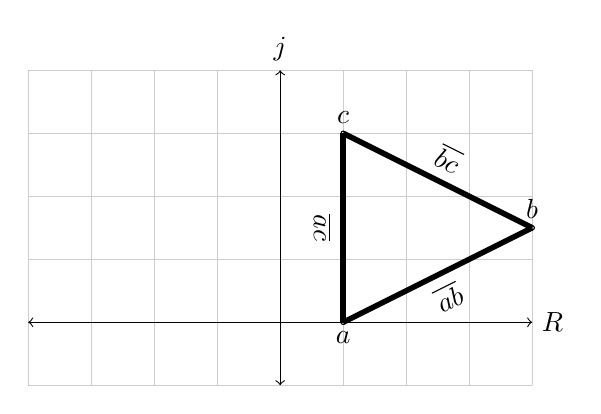
\begin{tikzpicture}[scale=0.8]
    \draw [thin,gray!40] (-4,-1) grid (4,4);
    \draw[<->] (-4,0)--(4,0) node[right] {$R$};
    \draw[<->] (0,-1)--(0,4) node[above]{$j$};
    \coordinate (a) at (1,0);
    \coordinate (b) at (4,1.5);
    \coordinate (c) at (1,3);
   
    \draw[black] (a) circle(1pt) node[anchor=north]{$a$};
    \draw[black] (b) circle(1pt) node[anchor=south]{$b$};
    \draw[black] (c) circle(1pt) node[anchor=south]{$c$};
    \draw[line width=2pt,black,-] (a)--(b) node[midway, below, sloped]{$\overline{ab}$};
    \draw[line width=2pt,black,-] (b)--(c) node[midway, above, sloped]{$\overline{bc}$};
    \draw[line width=2pt,black,-] (c)--(a) node[midway, below, sloped]{$\overline{ac}$};
\end{tikzpicture}
\caption*{Triangulo $s$}
    \end{minipage}
    \begin{minipage}{0.49\textwidth}
    \centering
        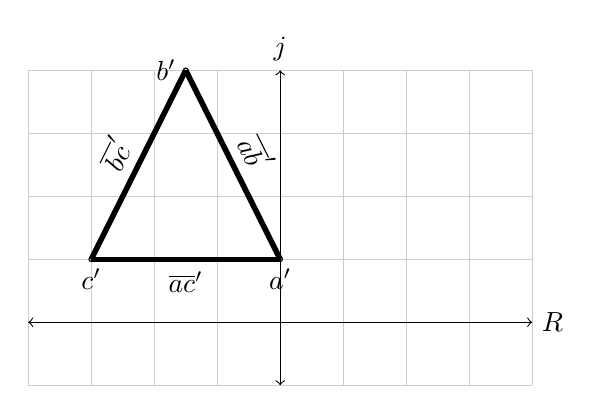
\begin{tikzpicture}[scale=0.8]
    \draw [thin,gray!40] (-4,-1) grid (4,4);
    \draw[<->] (-4,0)--(4,0) node[right] {$R$};
    \draw[<->] (0,-1)--(0,4) node[above]{$j$};
    \coordinate (1) at (0,1);
    \coordinate (2) at (-1.5,4);
    \coordinate (3) at (-3,1);
   
    \draw[black] (1) circle(1pt) node[anchor=north]{$a'$};
    \draw[black] (2) circle(1pt) node[anchor=east]{$b'$};
    \draw[black] (3) circle(1pt) node[anchor=north]{$c'$};
    \draw[line width=2pt,black,-] (1)--(2) node[midway, above, sloped]{$\overline{ab}'$};
    \draw[line width=2pt,black,-] (2)--(3) node[midway, above, sloped]{$\overline{bc}'$};
    \draw[line width=2pt,black,-] (3)--(1) node[midway, below, sloped]{$\overline{ac}'$};
\end{tikzpicture}
\caption*{Mapeo del triangulo $s$}
    \end{minipage}
    \caption{}
    \label{fig:RotF1}
\end{figure}
\begin{figure}[H]
    \centering
    \begin{tikzpicture}
    \draw [thin,gray!40] (-6,-2) grid (6,6);
    \draw[<->] (0,-2)--(0,6) node[anchor=south east]{$R'$};
    \draw[<->] (-6,0) node[left] {$j'$}--(6,0);
    \draw[mlgb,dashed] (-6,0)--(6,0) node[right] {$R$} ;
    \draw[mlgb,dashed] (0,-2)--(0,6) node[anchor=south west]{$j$};
    \coordinate (a) at (1,0);
    \coordinate (b) at (4,1.5);
    \coordinate (c) at (1,3);
    \coordinate (1) at (0,1);
    \coordinate (2) at (-1.5,4);
    \coordinate (3) at (-3,1);
   
    \draw[mlgb] (a) circle(1pt) node[anchor=north]{$a$};
    \draw[mlgb] (b) circle(1pt) node[anchor=south]{$b$};
    \draw[mlgb] (c) circle(1pt) node[anchor=south]{$c$};
    \draw[black] (1) circle(1pt) node[anchor=north]{$a'$};
    \draw[black] (2) circle(1pt) node[anchor=east]{$b'$};
    \draw[black] (3) circle(1pt) node[anchor=north]{$c'$};
    \draw[line width=1pt,mlgb,-] (a)--(b) node[midway, below, sloped]{$\overline{ab}$};
    \draw[line width=1pt,mlgb,-] (b)--(c) node[midway, above, sloped]{$\overline{bc}$};
    \draw[line width=1pt,mlgb,-] (c)--(a) node[midway, below, sloped]{$\overline{ac}$};
    \draw[line width=2pt,black,-] (1)--(2) node[midway, above, sloped]{$\overline{ab}'$};
    \draw[line width=2pt,black,-] (2)--(3) node[midway, above, sloped]{$\overline{bc}'$};
    \draw[line width=2pt,black,-] (3)--(1) node[midway, below, sloped]{$\overline{ac}'$};
    \draw[line width=1pt,black,dotted] (a) arc (0:90:1) ;
    \draw[line width=1pt,black,dotted] (b) arc (20.556:110.556:4.272) ;
    \draw[line width=1pt,black,dotted] (c) arc (71.565:161.565:3.1623) ;
    \draw[line width=1pt,black,dotted] (6,0) arc (0:90:6) ;
    \draw[line width=1pt,black,dashed] (0,6) arc (90:180:6) ;
\end{tikzpicture}
\caption{Plano $w$ graficado sobre el plano $z$ siendo $f_{z}$ un rotación}
    \label{fig:RotF3}
\end{figure}
\unsubsection{Funciones lineales}
Una función lineal es aquella que se describe como una suma de las funciones desplazamiento, escalado y dependiendo del factor de escalado una rotación. Se define una función lineal en un plano complejo como:
\begin{equation}
    w=f_{(z)}\lrah w=\lambda z+z_0
\end{equation}
Si $\lambda$ es un numero complejo, la ampliación con lleva una rotación. El mapeo de una curva entonces se puede realizar aplicando de forma progresiva las transformaciones. Primero la rotación, luego la ampliación y por ultimo el desplazamiento. Siempre se deben aplicar las transformaciones a las curvas afectadas por la ultima transformación. Se le por ejemplo plantemos el disco:
\begin{equation}
    \Vec{a}=re^{j\theta}+z_0\begin{cases}
        1\leq r\leq1.5\\
        z_0=(1+j0)
    \end{cases}
\end{equation}
\begin{figure}[H]
    \centering
    \begin{tikzpicture}[scale=0.7]
    \draw[thin,gray!40] (-4,-4) grid (4,4);
    \draw[<->] (-4,0)--(4,0) node[right] {$R$};
    \draw[<->] (0,-4)--(0,4) node[above]{$j$};
    \coordinate (a) at (1,0);
    \fill[fill=mlgb, fill opacity=0.6,even odd rule] (a) circle (1.5) (a) circle (1);
    \draw[fill=black] (a) circle(2pt) node[anchor=north east]{$z_0$};
    \draw [black,line width=2pt](a) circle (1);
    \draw [black,line width=2pt](a) circle (1.5);
\end{tikzpicture}
\caption{Disco en el plano complejo}
    \label{fig:LinF1}
\end{figure}
Y le aplicamos la transformación:
\begin{equation}
    w=f_(z)\lrah w=j2\cdot z-(-1+j)
\end{equation}
Entonces primero le aplicaríamos la rotación
\begin{equation}
    \vec{a}'=re^{j\theta}+j\begin{cases}
        1\leq r\leq1.5\\
    \end{cases}
\end{equation}
Como vemos, al ser un disco nuestra curva, la rotación solo afecto su centro. El argumento al estar acotado entre $pi$ y $-pi$, sumarle un $\frac{\pi}{2}$, correspondiente a la rotación, no con lleva afectar el modulo del intervalo, seguirá siendo un intervalo de modulo $2\pi$, entonces el disco seguirá siendo un disco completo. 

Luego le aplicamos la ampliación:
\begin{equation}
    \vec{\hat{a}}=2re^{j\theta}+2j\begin{cases}
        1\leq r\leq1.5\\
    \end{cases}
\end{equation}
Y por ultimo el desplazamiento:
\begin{equation}
     \vec{\hat{a}}'=2re^{j\theta}(1+j)\begin{cases}
        1\leq r\leq1.5\\
    \end{cases}
\end{equation}
\begin{figure}[H]
    \centering
    \begin{minipage}{0.29\textwidth}
    \centering
        \begin{tikzpicture}[scale=0.4]
    \draw[thin,gray!40] (-5,-5) grid (5,5);
    \draw[<->] (-5,0)--(5,0) node[right] {$R$};
    \draw[<->] (0,-5)--(0,5) node[above]{$j$};
    \coordinate (a) at (0,1);
    
    \fill[fill=mlgb, fill opacity=0.6,even odd rule] (a) circle (1.5) (a) circle (1);
    \draw[fill=black] (a) circle(2pt) node[anchor=north east]{$z_0$};
    \draw [black,line width=2pt](a) circle (1);
    \draw [black,line width=2pt](a) circle (1.5);
\end{tikzpicture}
\caption*{Rotación}

        \label{fig:LinRotF}
    \end{minipage}
    \begin{minipage}{0.29\textwidth}
    \centering
        \begin{tikzpicture}[scale=0.4]
    \draw[thin,gray!40] (-5,-5) grid (5,5);
    \draw[<->] (-5,0)--(5,0) node[right] {$R$};
    \draw[<->] (0,-5)--(0,5) node[above]{$j$};
    \coordinate (a) at (0,2);
    
    \fill[fill=mlgb, fill opacity=0.6,even odd rule] (a) circle (3) (a) circle (2);
    \draw[fill=black] (a) circle(2pt) node[anchor=north east]{$z_0$};
    \draw [black,line width=2pt](a) circle (2);
    \draw [black,line width=2pt](a) circle (3);
\end{tikzpicture}
\caption*{Ampliación}

        \label{fig:LinAmpF}
    \end{minipage}
    \begin{minipage}{0.29\textwidth}
    \centering
        \begin{tikzpicture}[scale=0.4]
    \draw[thin,gray!40] (-5,-5) grid (5,5);
    \draw[<->] (-5,0)--(5,0) node[right] {$R$};
    \draw[<->] (0,-5)--(0,5) node[above]{$j$};
    \coordinate (a) at (2,1);
    
    \fill[fill=mlgb, fill opacity=0.6,even odd rule] (a) circle (3) (a) circle (2);
    \draw[fill=black] (a) circle(2pt) node[anchor=north east]{$z_0$};
    \draw [black,line width=2pt](a) circle (2);
    \draw [black,line width=2pt](a) circle (3);
\end{tikzpicture}
\caption*{Desplazamiento}

        \label{fig:LinDesF}
    \end{minipage}
    \caption{}
\end{figure}
\begin{figure}[H]
    \centering
    \begin{tikzpicture}
    \coordinate (a) at (1,0);
    \draw[fill=mlgb] (a) circle(2pt) node[anchor=north west]{$z_0$};
    
    \draw[thin,mlgb] (-5,-5) grid (5,5);
    %\draw[step=2,line width=0.75pt,black] (-5,-5) grid (5,5);
    \draw[line width=0.75pt,black, dashed] (-5,0)--(5,0) node[right] {$R$};
    \draw[line width=0.75pt,black, dashed] (0,-5)--(0,5) node[above]{$j$};
    \draw[line width=1.5pt,<->] (-5,-1) node[left] {$j'$} --(5,-1) ;
    \draw[line width=1.5pt,<->] (1,-5)--(1,5) node[above]{$R'$};
    
    \coordinate (1) at (2,1);

    \fill[fill opacity=0.6, pattern=north east lines, pattern color=mlgb, even odd rule] (a) circle (1.5) (a) circle (1);
    
    \draw [mlgb,line width=1pt](a) circle (1);
    \draw [mlgb,line width=1pt](a) circle (1.5);
    
    \fill[fill=mlgb, fill opacity=0.6,even odd rule] (1) circle (3) (1) circle (2);
    \draw[fill=black] (1) circle(2pt) node[anchor=south west]{$z_0'$};
    \draw [black,line width=2pt](1) circle (2);
    \draw [black,line width=2pt](1) circle (3);
\end{tikzpicture}
\caption{Plano $w$ graficado sobre el plano $z$ siendo $f_{z}$ siendo una funcion lineal}
    \label{fig:}
\end{figure}